% documentclass[a4paper,12pt]{article}
\documentclass[a4paper,12pt]{ctexrep}
\usepackage{amsmath, amssymb}
\usepackage{hyperref}
\usepackage{graphicx} %插入图片的宏包
\usepackage{float} %设置图片浮动位置的宏包
\usepackage{subfigure} %插入多图时用子图显示的宏包


\begin{document}

\title{高数作业05.26}
\author{greenhandzdl}
\date{\today}
\maketitle

\pagenumbering{roman}
\tableofcontents
\newpage
\pagenumbering{arabic}

\part{A}
\section{试卷}

\begin{figure}[H] %H为当前位置,!htb为忽略美学标准,htbp为浮动图形
\centering %图片居中
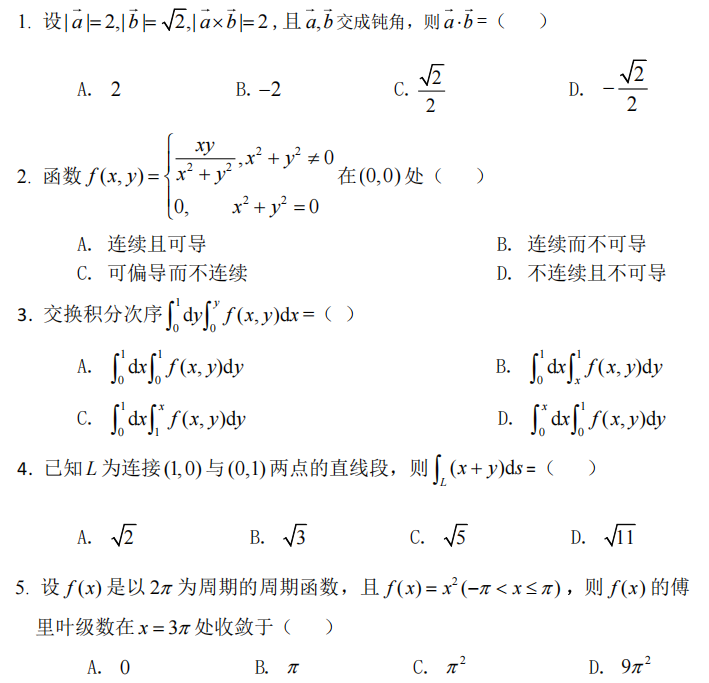
\includegraphics[width=1\textwidth]{20250526/1.png} %插入图片,[]中设置图片大小,{}中是图片文件名
\caption{选择题} %最终文档中希望显示的图片标题
\end{figure}

\begin{figure}[H]
\centering
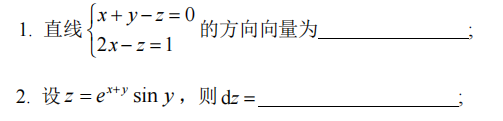
\includegraphics[width=1\textwidth]{20250526/2.png} 
\end{figure}
\begin{figure}[H]
	\centering
	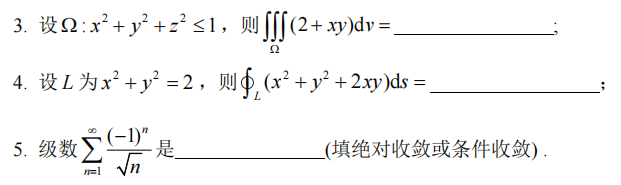
\includegraphics[width=1\textwidth]{20250526/3.png} 
	\caption{填空题} 
\end{figure}

\begin{figure}[H]
	\centering
	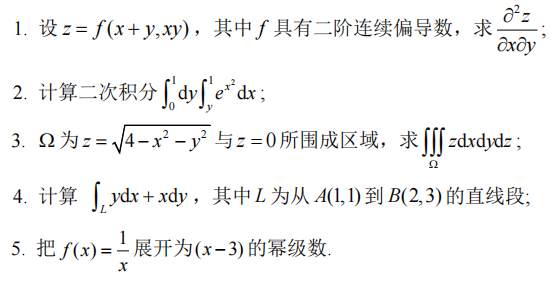
\includegraphics[width=1\textwidth]{20250526/4.png} 
\end{figure}
\begin{figure}[H]
	\centering
	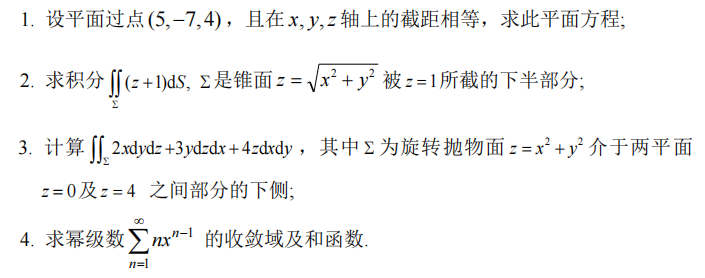
\includegraphics[width=1\textwidth]{20250526/5.png} 
\end{figure}
\begin{figure}[H]
	\centering
	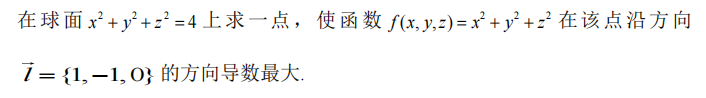
\includegraphics[width=1\textwidth]{20250526/6.png} 
\end{figure}
\begin{figure}[H]
	\centering
	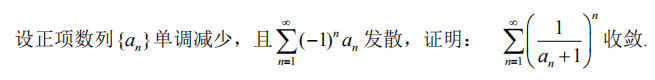
\includegraphics[width=1\textwidth]{20250526/7.png} 
	\caption{客观题} 
\end{figure}

\newpage
\part{B}
\section{作答}

\subsection{选择题1}
选\textbf{C}
\begin{equation*}
	\because\left(|\overrightarrow{a}||\overrightarrow{b}|\right)^2=\left(\overrightarrow{a}\cdot\overrightarrow{b}\right)^2+\left(\overrightarrow{a}\times\overrightarrow{b}\right)^2
\end{equation*}
\begin{equation*}
	\Leftrightarrow(2\sqrt{2})^{2}=2^{2}+(\overrightarrow{a}\cdot\overrightarrow{b})^{2}
\end{equation*}
\begin{equation*}
\therefore\overrightarrow{a}-\overrightarrow{b}=\pm2
\end{equation*}
\begin{equation*}
\begin{aligned}\because<\overrightarrow{a},\overrightarrow{b}>>\frac{\pi}{2}
		\\
\therefore\overrightarrow{a}\cdot\overrightarrow{b}=-2\end{aligned}\end{equation*}

\subsubsection{选择题2}
选\textbf{D} \\
由不等式链:
\begin{equation*}
\frac{2}{\frac{1}{a}+\frac{1}{b}}\leq\sqrt{ab}\leq\frac{a+b}{2}\leq\sqrt{\frac{a^{2}+b^{2}}{2}}
\end{equation*}
\begin{equation*}
	a^{2}+b^{2}\geq2ab
\end{equation*}
\begin{equation*}
	\operatorname*{lim}_{(x,y)\rightarrow(0,0)}\frac{xy}{x^2+y^2}\leq\frac{1}{2}
\end{equation*}
所以不连续,也不可导(不在$\mathbb{R}$上可微)

\subsubsection{选择题3}
选\textbf{B} \\
画图,得到范围

\subsubsection{选择题4}
选\textbf{A} \\
显然,直线\begin{equation*}
	x+y-1=0,0\leq x\leq1
\end{equation*}
\begin{equation*}
	\because y=1-x\therefore\frac{dy}{dx}=-1
\end{equation*}
\begin{equation*}
\therefore\int_{L}(x+y)ds=\int_{0}^{1}1\cdot\sqrt{1+(-1)^{2}}dx=\sqrt{2}
\end{equation*}

\subsubsection{选择题5}
选\textbf{C} \\
周期延拓就行了,下面不需要.
\begin{equation*}
\begin{aligned}
\because a_{n}=\int_{-\pi}^{\pi}f(x)\cos(n\pi x)dx,b_{n}=\int_{-\pi}^{\pi}f(x)\sin(n\pi x)dx \\
\therefore 
a_{n}=,
b_{n}=0
\end{aligned}
\end{equation*}

\newpage

\subsection{填空题1}
\textbf{(-1,-1,-2)}
\begin{equation*}
(1,1,-1)\times(2,0,-1) =(-1,-1,-2)
\end{equation*}

\subsubsection{填空题2}
\textbf{$e^{x+y}\sin y \cdot dx + e^{x+y} (\sin y + \cos y ) \cdot dy$}
\begin{equation*}
\begin{aligned}dz&=d(e^{x+y}\sin y)=d(e^{x+y})\sin y+\cos y\cdot e^{x+y}dy\\&
=e^{x+y}\sin y(dx+dy)+\cos ye^{x+y}dy\\&
=e^{x+y}\sin y \cdot dx + e^{x+y} (\sin y + \cos y ) \cdot dy
\end{aligned}
\end{equation*}

\subsubsection{填空题3}
\textbf{$\frac{8}{3}\pi$}

不妨将被积函数分为$$f(x,y,z)=2,g(x,y,z)=xy$$,显然对$f(x,y,z)$积分得到两倍体积的大小.$g(x,y,z)$是分别与x和y相关的奇函数,这个得出来的结果显然为0.
那么,我们只需要对$f(x,y,z)$积分就行了.
\begin{equation*}{2\iiint_{w}dv=2(\frac{4}{3}\cdot\pi\cdot 1^{2})=\frac{8}{3}\pi }\end{equation*}

\subsubsection{填空题4}
\textbf{$4 \sqrt{2} \pi $}

不妨转化为极坐标,注意到:$\theta\in[0,2\pi],\rho=\sqrt{2}$,所以原式=\begin{equation*}
	\oint_{0}^{2\pi}\left(2+4\sin\theta\cos\theta\right)\cdot\sqrt{2}d\theta = 4 \sqrt{2} \pi
\end{equation*}

\subsubsection{填空题5}
\textbf{相对收敛}

注意到$\sum_{n=1}^{\infty}{\frac{(-1)^{n}}{\sqrt{n}}}$的正向级数是p-级数,发散.所以是相对收敛

\newpage

\subsection{客观题组1}
\subsubsection{客观题1}
\begin{eqnarray*}
	\frac{\partial z}{\partial x}=f_{1}+f_{2}y \\
	\frac{\partial z}{\partial x\partial y}=f_{11}+f_{12}x+f_{21}y+f_{22}xy+f_{2}
\end{eqnarray*}

\subsubsection{客观题2}
这是一个很显然的转变积分区域的题目,可以由\begin{equation*}
	\int_{0}^{1}dy\int_{y}^{1}e^{x^{2}}dx
	=\int_{0}^{1}dx\int_{0}^{x}e^{x^{2}}dy
	=\frac{e - 1}{2}
\end{equation*}

\subsubsection{客观题3}
\newcounter{counter1}
\setcounter{counter1}{1}
$\omega$是$\Omega$的第\Roman{counter1}象限的子空间.显然,$$\begin{aligned}r&=2\\\theta&\in[0,\pi]\end{aligned}$$
\begin{equation*}
	 \begin{aligned}& \therefore \iiint_{\Omega}z\mathrm{dxdydz} \\&
 =4\iiint_{\omega}z\mathrm{dxdydz} \\&
 =4\int_{0}^{1}zdz\int_{0}^{\frac{\pi}{2}}d\theta\int_{0}^{2}rdr\\&
	=\frac{1}{2}\times\frac{\pi}{2}\times\frac{2^{2}}{2}\times4\\&
	=2\pi\end{aligned}
\end{equation*}

\subsubsection{客观题4}
$$\because(y)^{\prime}_y=(x)^{\prime}_y$$,我们可以知道其路径无关. \\
注意:Green公式$\oint_{\partial D}P\mathrm{d}x+Q\mathrm{d}y=\iint_{D}\left(\frac{\partial Q}{\partial x}-\frac{\partial P}{\partial y}\right)\mathrm{d}x\mathrm{d}y$. \\
我们不妨考虑路径先沿着x移动,再沿着y移动.
\begin{equation*}
\begin{aligned}&\int_{L}ydx+xdy\\&
	=(xy)|_{x\in(1,2),y=1}+(xy)_{x=2,y\in(1,3)}\\&
	=1+4\\&
	=5\end{aligned}
\end{equation*}

\subsubsection{客观题5}
$$ \because f(x)=\frac{1}{x}=\frac{1}{3+(x-3)}=\frac{1}{3}\cdot\frac{1}{1+\frac{1}{3}(x-3)} $$
我们可以根据公式$\frac{1}{1+x}=\sum_{n=0}^\infty(-1)^nx^n=1-x+x^2-x^3+\cdots+(-1)^nx^n+\cdots,x\in(-1,1)$进行展开. 
$$ \therefore f(x) = \sum_{n=0}^\infty
(-1)^{n} (\frac{1}{3})^{n+1} \cdot (x-3)^{n} $$ 

\newpage

\subsection{客观题组2}
\subsubsection{客观题1}
显然,截距不为0.设
$$ \frac{x + y + z}{a} = 1 $$,代入坐标$(5,-7,4)$,解得$a=2$,所以方程式是$$x+y+z-2=0$$

\subsubsection{客观题2}
投影到XoY面上,有
$$\iint_Sf(x,y,z)ds=\iint_{D_{xy}}f(x,y,z(x,y))\sqrt{(z_x^{^{\prime}})^2+(z_y^{^{\prime}})^2+1}dxdy$$
显然,投影面$x^{2} + y^{2} \leq  1$ \\
那么,原式=$$\iint_{D_{xy}}(\sqrt{x^{2}+y^{2}}+1)\sqrt{\frac{x^{2}+y^{2}}{x^{2}+y^{2}}+1}d\sigma = \iint_{D_{xy}}(\sqrt{x^{2}+y^{2}}+1)\sqrt{2}d\sigma
=\sqrt{2}\int_{0}^{2\pi}d\theta\int_{0}^{1}\rho(1+\rho)d\rho$$
$\therefore $原式=$\frac{5 \sqrt{2} \pi}{3}$



\subsubsection{客观题3}
高斯公式:$\iiint_{\Omega}(\frac{\partial P}{\partial x}+\frac{\partial Q}{\partial y}+\frac{\partial R}{\partial z})dv=\iint_{\Sigma}Pdydz+Qdzdx+Rdxdy$
那么有:
$$\oint_{\sum-\sum_{1}}2xdydz+3ydzdx+4zdxdy=9\int\int\int_{\omega}dv-16\int\int_{\sum_{1}}dxdy$$
对于Dxy面投影,有$x^{2}+y^{2}\leq4$
对于空间$\omega$,有
$$\begin{cases}0\leq \theta\leq\sqrt{z}\\0\leq\theta\leq2\pi\\0\leq z\leq4&\end{cases}$$
$\therefore$ 原式= $9\int_{0}^{4}dz\int_{0}^{2\pi}d\theta\int_{0}^{\sqrt{z}}\rho d\rho-16\int_{0}^{2\pi}d\theta\int_{0}^{2}\rho dp$\\
$\therefore$ 原式$=8\pi$

\subsubsection{客观题4}
注意到$$S(x)=\sum_{n=1}^{\infty}nx^{n-1}=(\sum_{n=1}^{\infty}x^{n})^{\prime}=(\frac{1}{1-x})^{\prime}=\frac{1}{(1-x)^{2}}$$
根据$\lim_{n\to+\infty}\frac{(n+1)x^{n}}{nx^{n-1}}=\frac{n+1}{n}x<1$知道收敛域$x \in (-1,1)$

\newpage

\subsection{客观题组3}
显然,求梯度,再根据单位方向向量计算.
$$\overrightarrow{\nabla}=\begin{bmatrix}2x\\2y\\2z\end{bmatrix}$$
$$\overrightarrow{e_{l}}=\frac{l}{|l|}=\begin{bmatrix}\frac{\sqrt{2}}{2}\\-\frac{\sqrt{2}}{2}\\0\end{bmatrix}$$
不妨设$\theta,\phi \in [0,2\pi]$:
$$\begin{cases}x=2\cos\theta\cos \phi\\y=2\cos\theta\sin \phi\\z=2\sin\theta&\end{cases}$$
代入$\overrightarrow{\nabla}  \cdot \overrightarrow{e_{l}}$得到:
$$ f(\theta,\phi) = \sqrt{2} cos\theta\cdot (cos \phi - sin \phi )$$
注意到$ \theta = 0, \phi = \frac{7\pi}{4} $时,最大.解得:
$$\begin{bmatrix}\sqrt{2} \\ -\sqrt{2} \\0\end{bmatrix}$$

\newpage

\subsection{证明题}
显然$\operatorname*{lim}_{n\rightarrow+\infty}a_{n}\neq0$
根据柯西判别式:
\begin{equation*}
	\operatorname*{lim}_{n\rightarrow+\infty}\sqrt{(\frac{1}{1+a_{n}})^{n}}=\operatorname*{lim}_{n\rightarrow+\infty}\frac{1}{1+a_{n}}  < 1
\end{equation*}
$\therefore \sum_{n=1}^\infty\left(\frac{1}{a_n+1}\right)^n$收敛
\end{document}